% !TeX root = main.tex

\section{Sub-figures}

A figure can be composed of sub-figures as shown in Figure \ref{fig:f1-float}.

\begin{figure}
    \centering
    % Sub-Figures using subcaption
    \begin{subfigure}[b]{0.3\textwidth}
        \centering
        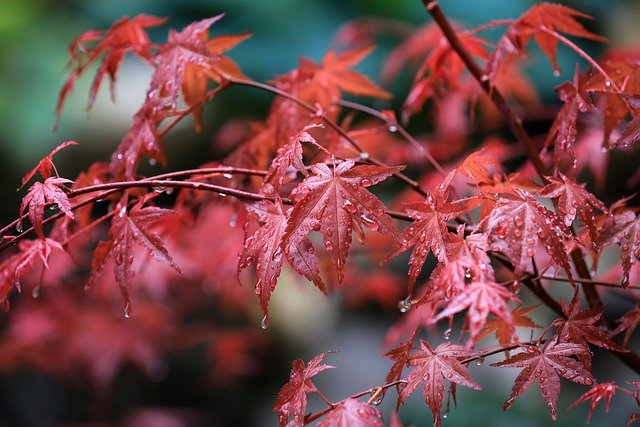
\includegraphics[width=\textwidth]{img3-1.jpg}
        \caption[Maple Leaves]{\href{https://pixabay.com/photos/maple-maple-leaves-raindrops-6290891/}{ilyessuti}}
        \label{fig:sfig-f1-1}
    \end{subfigure}
    % This is to put a space (even filling)
    \hfill
    \begin{subfigure}[b]{0.3\textwidth}
        \centering
        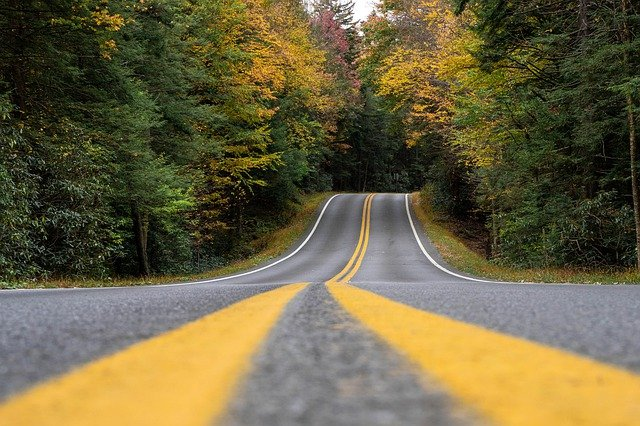
\includegraphics[width=\textwidth]{img3-2.jpg}
        \caption[Road]{\href{https://pixabay.com/photos/road-landscape-autumn-highway-fall-6745746/}{jatocreate}}
        \label{fig:sfig-f1-2}
    \end{subfigure}
    \hfill
    \begin{subfigure}[b]{0.3\textwidth}
        \centering
        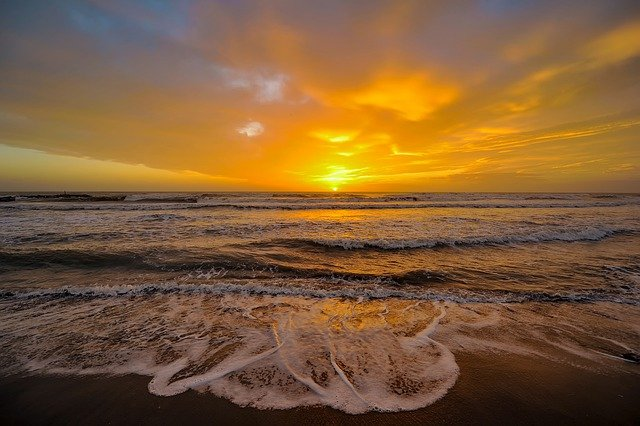
\includegraphics[width=\textwidth]{img3-3.jpg}
        \caption[Sunset]{\href{https://pixabay.com/photos/sunset-beach-sea-waves-shore-sand-6387462/}{lillolillolillo}}
        \label{fig:sfig-f1-3}
    \end{subfigure}
    \caption[Sub-Figures]{Simple 3 column 1 row figures}
    \label{fig:f1-float}
    \small
        The figure \ref{sub@fig:sfig-f1-1} is of maple leaves, figure \ref{sub@fig:sfig-f1-2} is of a road and figure \ref{sub@fig:sfig-f1-3} is of a sunset
\end{figure}

\subsection{More sub-figures}
A more complex sub-figures is shown in Figure \ref{fig:f2-float}.

\begin{figure}
    \centering
    \begin{subfigure}[b]{0.3\textwidth}
        \centering
        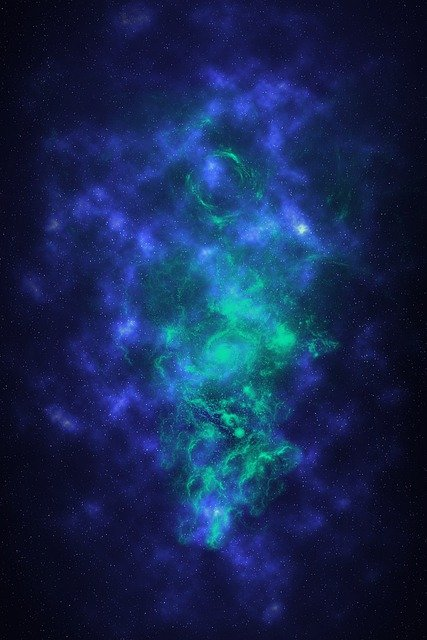
\includegraphics[width=\textwidth]{Complex-Sfig/img1.jpg}
        \caption[Space Art]{\href{https://pixabay.com/illustrations/space-art-space-abstract-galaxy-5626853/}{Slava\_Ivanov}}
    \end{subfigure}
    \begin{subfigure}[b]{0.3\textwidth}
        \centering
        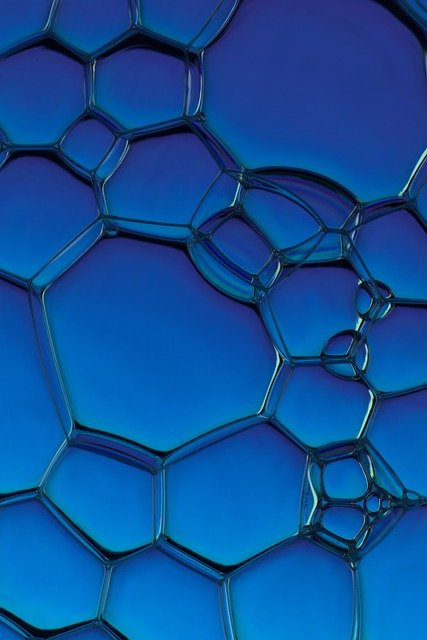
\includegraphics[width=\textwidth]{Complex-Sfig/img2.jpg}
        \caption[Template]{\href{https://pixabay.com/photos/background-colour-template-contrast-5074889/}{robert1029}}
    \end{subfigure}
    \begin{subfigure}[b]{0.3\textwidth}
        \centering
        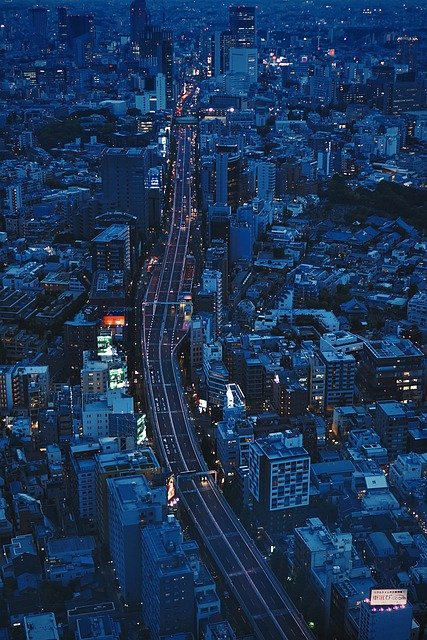
\includegraphics[width=\textwidth]{Complex-Sfig/img3.jpg}
        \caption[City]{\href{https://pixabay.com/photos/city-night-bird-s-eye-view-5644601/}{yeyalpha}}
    \end{subfigure}
    \begin{subfigure}[b]{0.5\textwidth}
        \centering
        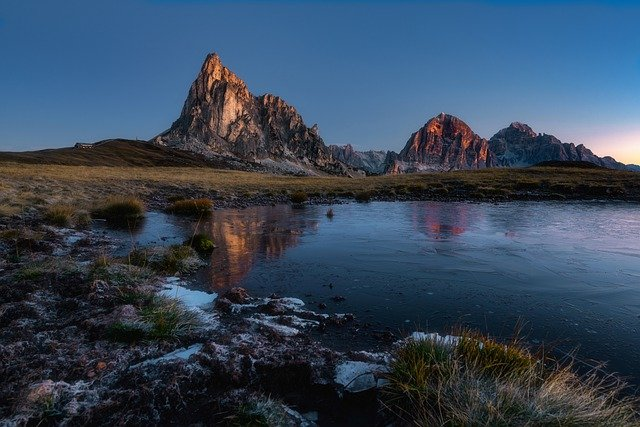
\includegraphics[width=\textwidth]{Complex-Sfig/img4.jpg}
        \caption[Mountains]{\href{https://pixabay.com/photos/italy-mountains-sunrise-nature-6728318/}{IdaT}}
    \end{subfigure}
    \newline
    \begin{subfigure}[b]{0.3\textwidth}
        \centering
        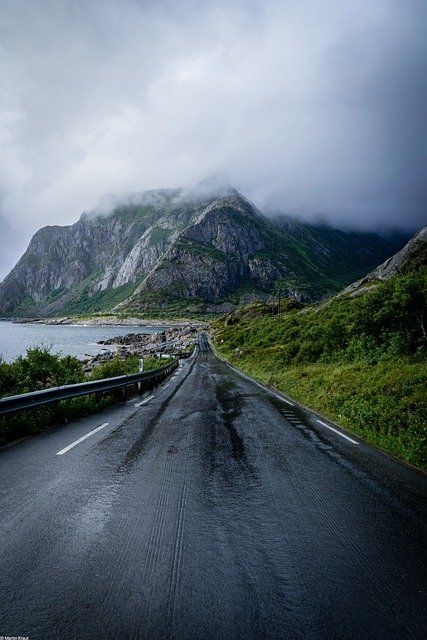
\includegraphics[width=\textwidth]{Complex-Sfig/img5.jpg}
        \caption[Road]{\href{https://pixabay.com/photos/road-highway-sea-mountains-coast-6597404/}{MartinKra}}
    \end{subfigure}
    \begin{subfigure}[b]{0.6\textwidth}
        \centering
        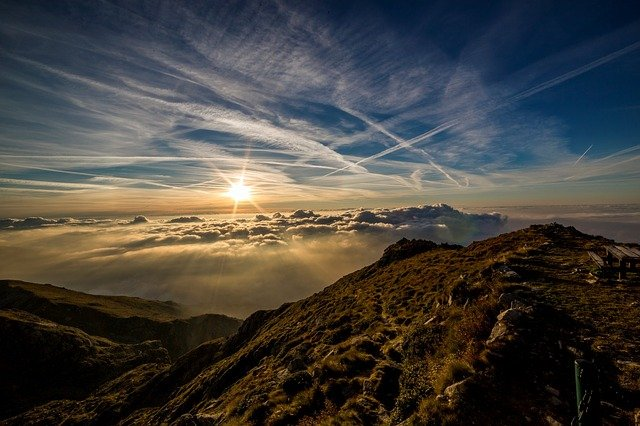
\includegraphics[width=\textwidth]{Complex-Sfig/img6.jpg}
        \caption[Mountains]{\href{https://pixabay.com/photos/mountains-sun-clouds-peak-summit-190055/}{danfador}}
    \end{subfigure}
    \caption{Different images}
    \label{fig:f2-float}
    \small
        It is demonstrated how you can create a layout from images
\end{figure}
